%!TEX program = xelatex

\documentclass[onecolumn,a4paper,10pt]{article}

\usepackage[ boldfont,slantfont]{xeCJK}  %设定支持中文
\usepackage{multicol}
\usepackage{array}
\usepackage{longtable}
\usepackage{color}
\usepackage{bbding}

\graphicspath{{figures/}}    %设置放置图片的文件夹

\linespread{1.2}     %设置行间距的命令

\setmainfont{Times New Roman}

%for windows fonts
%\setCJKmainfont[BoldFont={SimHei},ItalicFont={KaiTi}]{SimSun}
%\setsansfont{SimHei}
%
%\setCJKfamilyfont{song}{SimSun}
%\setCJKfamilyfont{kai}{KaiTi}
%\setCJKfamilyfont{hei}{SimHei}
%\setCJKfamilyfont{yao}{FZYaoTi}
%
%\newcommand\song{\CJKfamily{song}}
%\newcommand\kai{\CJKfamily{kai}}
%\newcommand\hei{\CJKfamily{hei}}
%\newcommand\yao{\CJKfamily{yao}}

\setCJKmainfont[BoldFont={STXihei},ItalicFont={STKaiti}]{STSong}
\setsansfont{STXihei}

\setCJKfamilyfont{song}{STSong}
\setCJKfamilyfont{kai}{STKaiti}
\setCJKfamilyfont{hei}{STXihei}
%\setCJKfamilyfont{yao}{FZYaoTi}

\newcommand\song{\CJKfamily{song}}
\newcommand\kai{\CJKfamily{kai}}
\newcommand\hei{\CJKfamily{hei}}
%\newcommand\yao{\CJKfamily{yao}}

\newcommand{\erhao}{\fontsize{22pt}{\baselineskip}\selectfont}
\newcommand{\xiaoerhao}{\fontsize{18pt}{\baselineskip}\selectfont}
\newcommand{\sanhao}{\fontsize{16pt}{\baselineskip}\selectfont}
\newcommand{\xiaosanhao}{\fontsize{15pt}{\baselineskip}\selectfont}
\newcommand{\sihao}{\fontsize{14pt}{\baselineskip}\selectfont}
\newcommand{\xiaosihao}{\fontsize{12pt}{\baselineskip}\selectfont}
\newcommand{\wuhao}{\fontsize{10.5pt}{\baselineskip}\selectfont}
\newcommand{\xiaowuhao}{\fontsize{9pt}{\baselineskip}\selectfont}
\newcommand{\liuhao}{\fontsize{7.5pt}{\baselineskip}\selectfont}

%%%段落首行缩进两个字
\makeatletter
\let\@afterindentfalse\@afterindenttrue
\@afterindenttrue
\makeatother
\setlength{\parindent}{2em}%中文缩进两个汉字位

\newcommand{\tabincell}[2]{\begin{tabular}{@{}#1@{}}#2\end{tabular}}

%%%%%%%%%% 定理类环境的定义 %%%%%%%%%%
%% 必须在导入中文环境之后
\newtheorem{example}{例}             % 整体编号
\newtheorem{algorithm}{算法}
\newtheorem{theorem}{定理}[section]  % 按 section 编号
\newtheorem{definition}{定义}
\newtheorem{axiom}{公理}
\newtheorem{property}{性质}
\newtheorem{proposition}{命题}
\newtheorem{lemma}{引理}
\newtheorem{corollary}{推论}
\newtheorem{remark}{注解}
\newtheorem{condition}{条件}
\newtheorem{conclusion}{结论}
\newtheorem{assumption}{假设}

%%%%%%%%%% 一些重定义 %%%%%%%%%%
%% 必须在导入中文环境之后
\renewcommand{\contentsname}{目录}     % 将Contents改为目录
\renewcommand{\abstractname}{摘\ \ 要} % 将Abstract改为摘要
\renewcommand{\refname}{参考文献}      % 将References改为参考文献
\renewcommand{\indexname}{索引}
\renewcommand{\figurename}{图}
\renewcommand{\tablename}{表}
\renewcommand{\appendixname}{附录}
%\renewcommand{\proofname}{证明}
\renewcommand{\algorithm}{算法}

%%%%%%%%%%%%%%%%%%%%%%%%%%%%%%%%%%%%%%%%%%%%%%%%%%%%%%%%%%%%%%%%
%  packages
%    这部分声明需要用到的包
%%%%%%%%%%%%%%%%%%%%%%%%%%%%%%%%%%%%%%%%%%%%%%%%%%%%%%%%%%%%%%%%
\usepackage{graphicx}    % EPS 图片支持
\usepackage{indentfirst} % 中文段落首行缩进
\usepackage{bm}          % 公式中的粗体字符(用命令\boldsymbol)
\usepackage{graphics}	%让文档支持图片
\usepackage{amsmath}	%ams可以让文档支持数学公式

\usepackage{fontspec,xunicode,xltxtra}
\usepackage{hyperref}	%让文档支持超链接
\usepackage{booktabs}	%让文档支持三线表格
\usepackage{amsfonts}
\usepackage{amssymb}
\usepackage{color}
\usepackage{graphicx,psfrag}
\usepackage{epsfig}
\usepackage{verbatim}
\usepackage{picins}
\usepackage{multirow}
\usepackage{listings}
\usepackage{xcolor}
\usepackage[titletoc]{appendix} %附件支持


%%%%%%%%%%%%%%%%%%%%%%%%%%%%%%%%%%%%%%%%%%%%%%%%%%%%%%%%%%%%%%%%
%  lengths
%    下面的命令重定义页面边距,使其符合中文刊物习惯。
%%%%%%%%%%%%%%%%%%%%%%%%%%%%%%%%%%%%%%%%%%%%%%%%%%%%%%%%%%%%%%%%
\addtolength{\topmargin}{-54pt}
\setlength{\oddsidemargin}{0.63cm}  % 3.17cm - 1 inch
\setlength{\evensidemargin}{\oddsidemargin}
\setlength{\textwidth}{14.66cm}
\setlength{\textheight}{24.00cm}    % 24.62
\begin{document}
%%%%%%%%%%%%%%%%%%%%%%%%%%%%%%%%%%%%%%%%%%%%%%%%%%%%%%%%%%%%%%%%
%  定义标题格式,包括title,author,affiliation,email等。
%  在任何用到中文的地方,用\begin{CJK} ... \end{CJK}将其括起来。
%%%%%%%%%%%%%%%%%%%%%%%%%%%%%%%%%%%%%%%%%%%%%%%%%%%%%%%%%%%%%%%%
\title{\hei{真空系统未来3个月器件统计和计划 }}
\author{肖波\footnote{xbustc@gmail.com}~~~~~~
\\[8pt]
\xiaowuhao 合肥微尺度物质科学国家实验室,安徽~~合肥~~230026\\[4pt]
}
%\date{\today}  % 这一行用来去掉默认的日期显示
\date{\today}
%%%%%%%%%%%%%%%%%%%%%%%%%%%%%%%%%%%%%%%%%%%%%%%%%%%%%%%%%%%%%%%%
%  自定义命令
%%%%%%%%%%%%%%%%%%%%%%%%%%%%%%%%%%%%%%%%%%%%%%%%%%%%%%%%%%%%%%%%
% 此行使文献引用以上标形式显示
\newcommand{\supercite}[1]{\textsuperscript{\cite{#1}}}
%%%%%%%%%%%%%%%%%%%%%%%%%%%%%%%%%%%%%%%%%%%%%%%%%%%%%%%%%%%%%%%%
%  显示title,并设页码为空(按杂志社要求)
%%%%%%%%%%%%%%%%%%%%%%%%%%%%%%%%%%%%%%%%%%%%%%%%%%%%%%%%%%%%%%%%
\maketitle
%\pagestyle{empty} \thispagestyle{empty}
\vspace{-20pt}

%%%%%%%%%%%%%%%%%%%%%%%%%%%%%%%%%%%%%%%%%%%%%%%%%%%%%%%%%%%%%%%%
%  中文摘要
%%%%%%%%%%%%%%%%%%%%%%%%%%%%%%%%%%%%%%%%%%%%%%%%%%%%%%%%%%%%%%%%

%\begin{center}
%\parbox{\textwidth}{
%\rule{2em}{0pt}
%\hei{摘要:}\song{在超冷原子相关的实验中,磁场的稳定性会极大的影响原子的退相干时间,因此,在大部分的超冷原子实验中都会配备PID反馈系统用以稳定原子的偏置磁场,延长相干时间。本方案基于海德堡光晶格实验室目前的方案,用以稳定原子的任意方向偏置磁场。}\\[5pt]
%\hei{关键词:}\song{很关键;很关键;非常关键}
%\\[5pt]
%}
%\end{center}



\iffalse
%%%%%%%%%%%%%%%%%%%%%%%%%%%%%%%%%%%%%%%%%%%%%%%%%%%%%%%%%%%%%%%%
%  英文摘要
%%%%%%%%%%%%%%%%%%%%%%%%%%%%%%%%%%%%%%%%%%%%%%%%%%%%%%%%%%%%%%%%
\begin{center}
\sihao{\textbf{A \LaTeX{} Template for Chinese Reports}}\\[7pt]
\normalsize
Weiyong Zhang~~~~~~
\\[7pt]
\xiaowuhao Hefei National Laboratory for Physical Sciences at the Microscale, HeFei, AnHui, 230026\\[10pt]
\end{center}
\begin{center}
\parbox{\textwidth}{
\textbf{Abstract:} This is a \LaTeX{} template used for writting documents in Chinese form.\\[4pt]
\textbf{Keywords:} Key; Key; the Key
}
\end{center}
\fi

\begin{figure}[htbp]
\centering
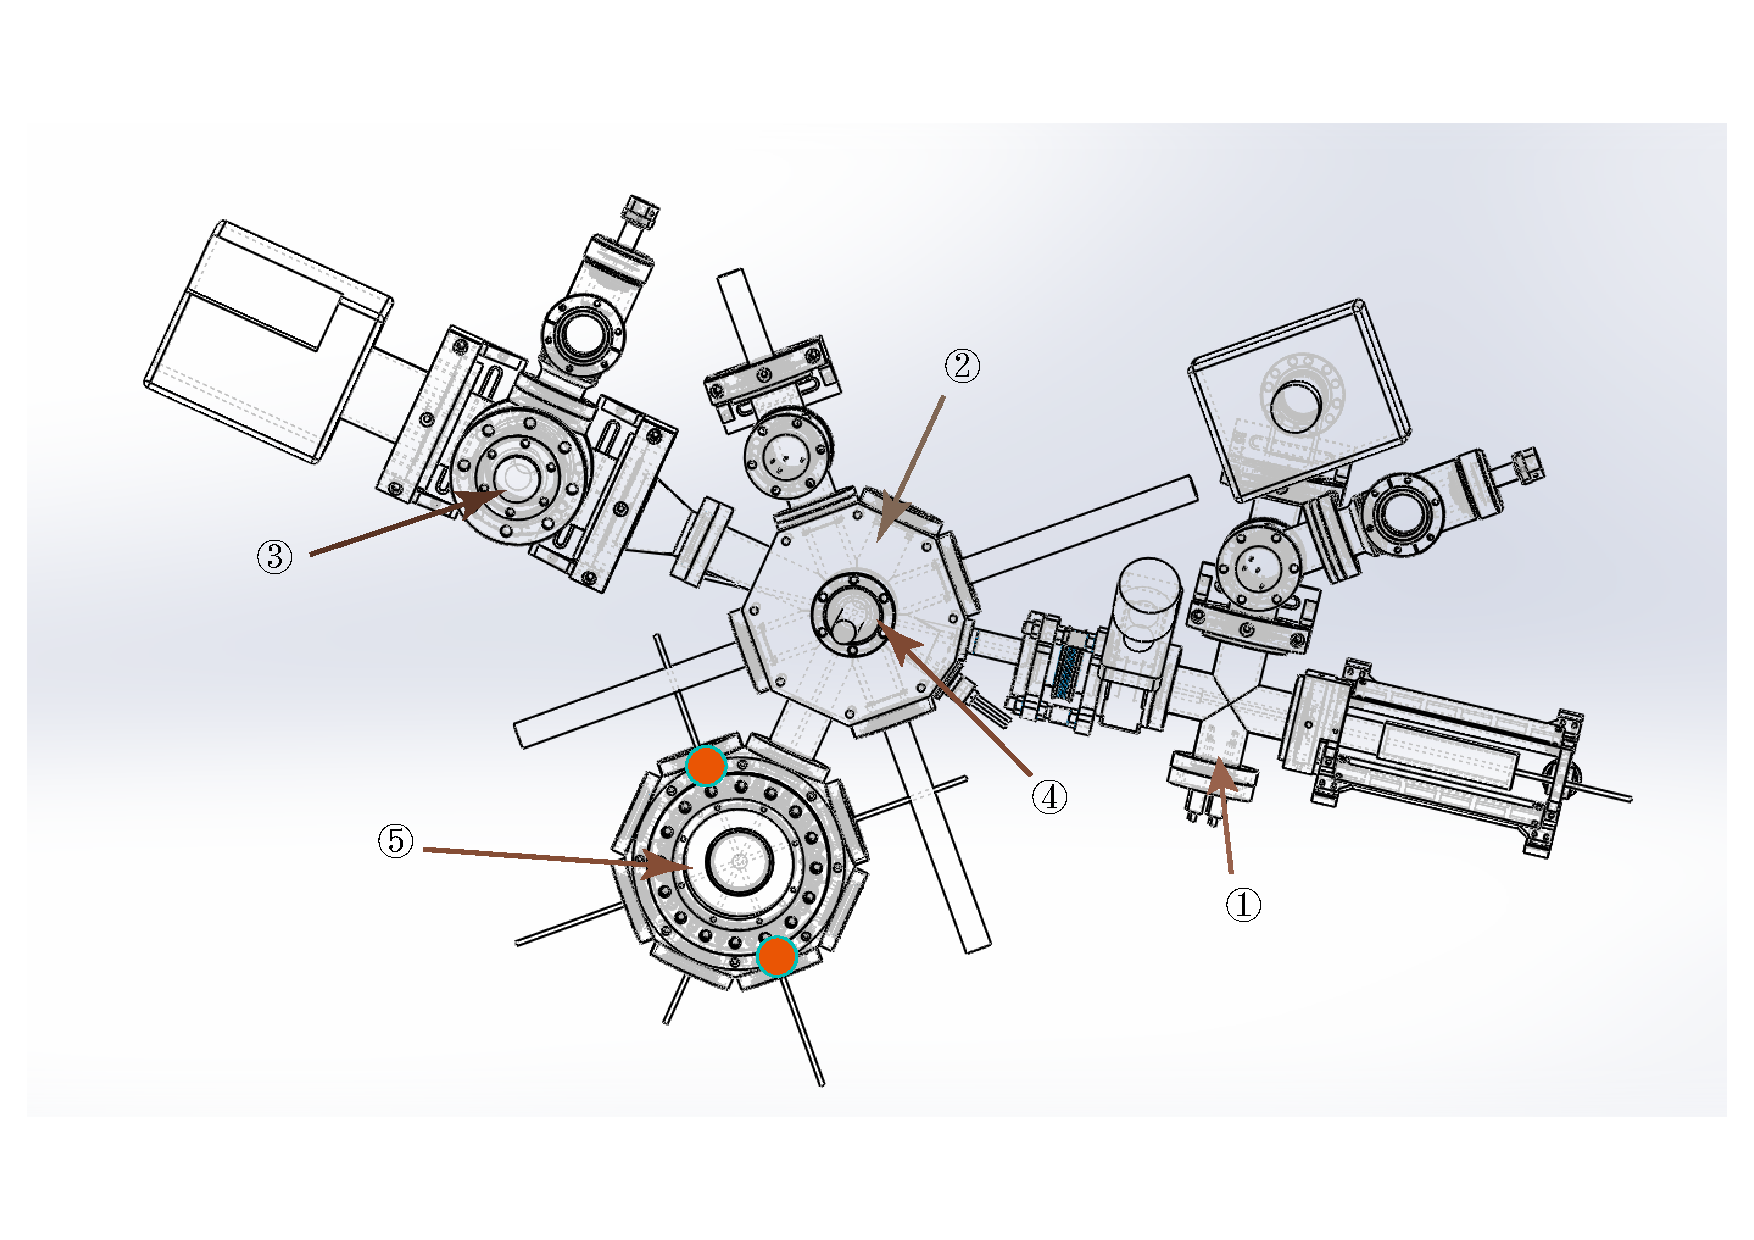
\includegraphics[width=0.7\textwidth]{真空图}
\caption{光晶格真空系统}
\label{fig:pict03-01}
\end{figure}

\section{更换器件统计和到货情况}


\begin{table}[htbp]


\label{tab:chap04-01}
\begin{tabular}{|c|c|c|c|c|c}
\hline
编号&器件& 到货情况&  Remarks\\
\hline
1 & Dispenser &  \tabincell{c}{3 dispensers from Alvatec and\\ 50 dispensers from SAES(已到)}&  \tabincell{c}{将安装2 dispensers from Alvatec \\和2 dispensers from SAES}\\
\hline
2 & 11-WAY & \tabincell{c}{1 chamber from Lesker (已到);\\磁补偿线圈框(未到)}&\\
\hline
3 & Titantium Sublimation Pump&Pump from Agilent (已到)&不需要更换控制器\\
\hline
4 & RF Coils&真空漆包线 from Lesker(已到)& \tabincell{c}{只需要用新买的真\\空漆包线重新绕一个即可}\\
\hline
5 &高分辨观察窗 & \tabincell{c}{From UKAEA(未到);\\磁补偿线圈框(已到)}&还需要打磨镀膜\\
\hline
&CF35观察窗 &From Lesker(已到)&\tabincell{c}{4块需要镀膜\\3块月底到货}\\
\hline
\end{tabular}
\end{table}




\section{安装规划}

以下是安装时的几个规划:
\begin{enumerate}
\item 真空平台最上层平台拆除,光路拆除.\Checkmark
\item 线切割扩大孔至半径80mm。
\item 第二层周围的光路拆除,拆除补偿线圈、MOT线圈和永磁铁架子。
\item 拆除MOT腔上的Transfer观察窗,把科学腔上的口用Lesker观察窗,UKAEA观察窗以及Transfer观察窗封上,对其捡漏。\textbf{\color{blue}同时,检查上下UKAEA观察窗M4螺纹孔是否在同一线上。}
\item 拆除玻璃腔,用Hositrad观察窗加上一个half nipple简单封上相应的口。将旧MOT腔拆除,将CF16的Feedthrough取下,用绝缘漆包线从新绕制RF Coil安装进11-way中,同时将旧MOT上的其他观察窗和Gauge安装到11-way上,并对其捡漏。
\item \textbf{\color{red}将一只激光笔固定在一个镜架上,将光斑高度调整到7cm。}
\item 拆除gate valve、Reducer、Port Aligner,更换差分出气管,用激光矫正reducer的中心和玻璃腔法兰面中心对准在7cm高度。
\item 用新的钛泵更换旧钛泵。
\item 将科学腔与11-way对接,用激光调节高度为7cm,并将整体固定在平台上,以科学腔的位置对准设计图设计位置为标准,再对整体捡漏。
\item 将钛泵段与11-way对接,捡漏。
\item 将分子泵和阀门连接,分子泵后端接检漏仪。
\item 将11-way与reducer对接,用激光检查是否光能从差分抽气管进入MOT腔,希望中心能都完整对好。
\item 安装dispenser并检查短路情况
\item 安装玻璃腔,并捡漏。
\end{enumerate}

\end{document}
